\definecolor{darkgreen}{rgb}{0.0, 0.5, 0.13}
\newcommand{\gct}{\color{darkgreen}\checkmark}
\newcommand{\rma}{\color{red}\ding{55}}
\newcommand{\bct}{\color{blue}\checkmark}

\author[Juan Cruz-Martinez]{}
\institute{University of Milan}

\subsection{Fitting the methodology}

\begin{frame}{Beyond the PDF fit: fitting the methodology}

    The main objective of NNPDF is to minimize choices that can bias the PDF:

    \begin{columns}
        \column{0.7\linewidth}
        \begin{itemize}
            \item[\rma] Functional form $\longrightarrow$ Neural Networks
            \item[\rma] However: NN are defined by set of parameters!
        \end{itemize}

        \vspace{0.2cm}

        Humans are good at recognising patterns but selecting the best
        set of parameters is a slow process and systematic success is not guaranteed
        \column{0.2\linewidth}
        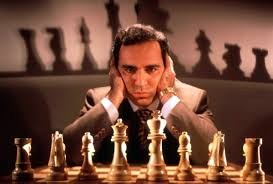
\includegraphics[width=\textwidth]{juan_future_hyperopt/kasparov.jpg}

        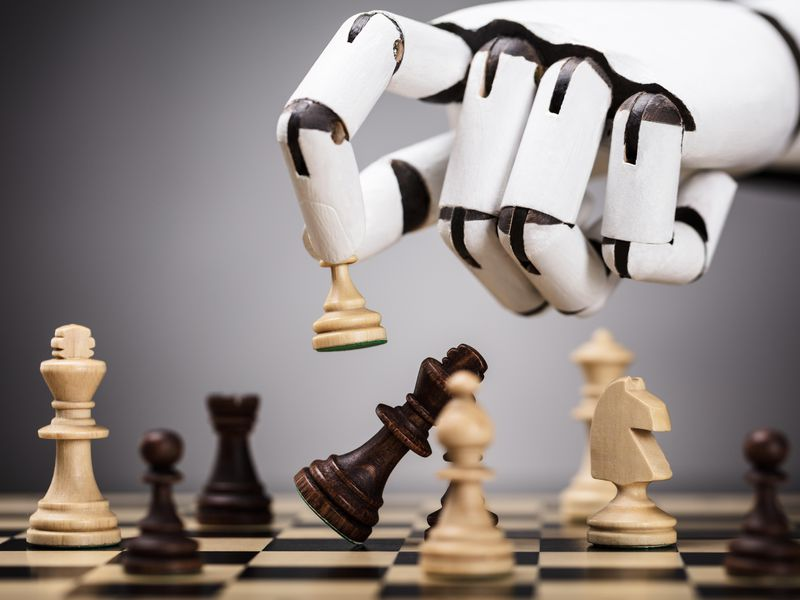
\includegraphics[width=\textwidth]{juan_future_hyperopt/alphazero.jpg}
        \column{0.1\linewidth}
    \end{columns}

    \vspace{0.2cm}

    To overcome this selection problem we implement a {\color{blue}  hyperparameter scan}: let the computer decide automatically

    \begin{itemize}
        \item[\gct] Scan over thousands of hyperparameter combinations
        \item[\gct] Define a reward function to grade the model
        \item[\gct] Check the genrealization power of the model
    \end{itemize}

\end{frame}

\begin{frame}
    \frametitle{Hyperparameter scan} 
    Each blue dot corresponds to a fit of a different set of hyperparameters:
    { 
        \centering 

        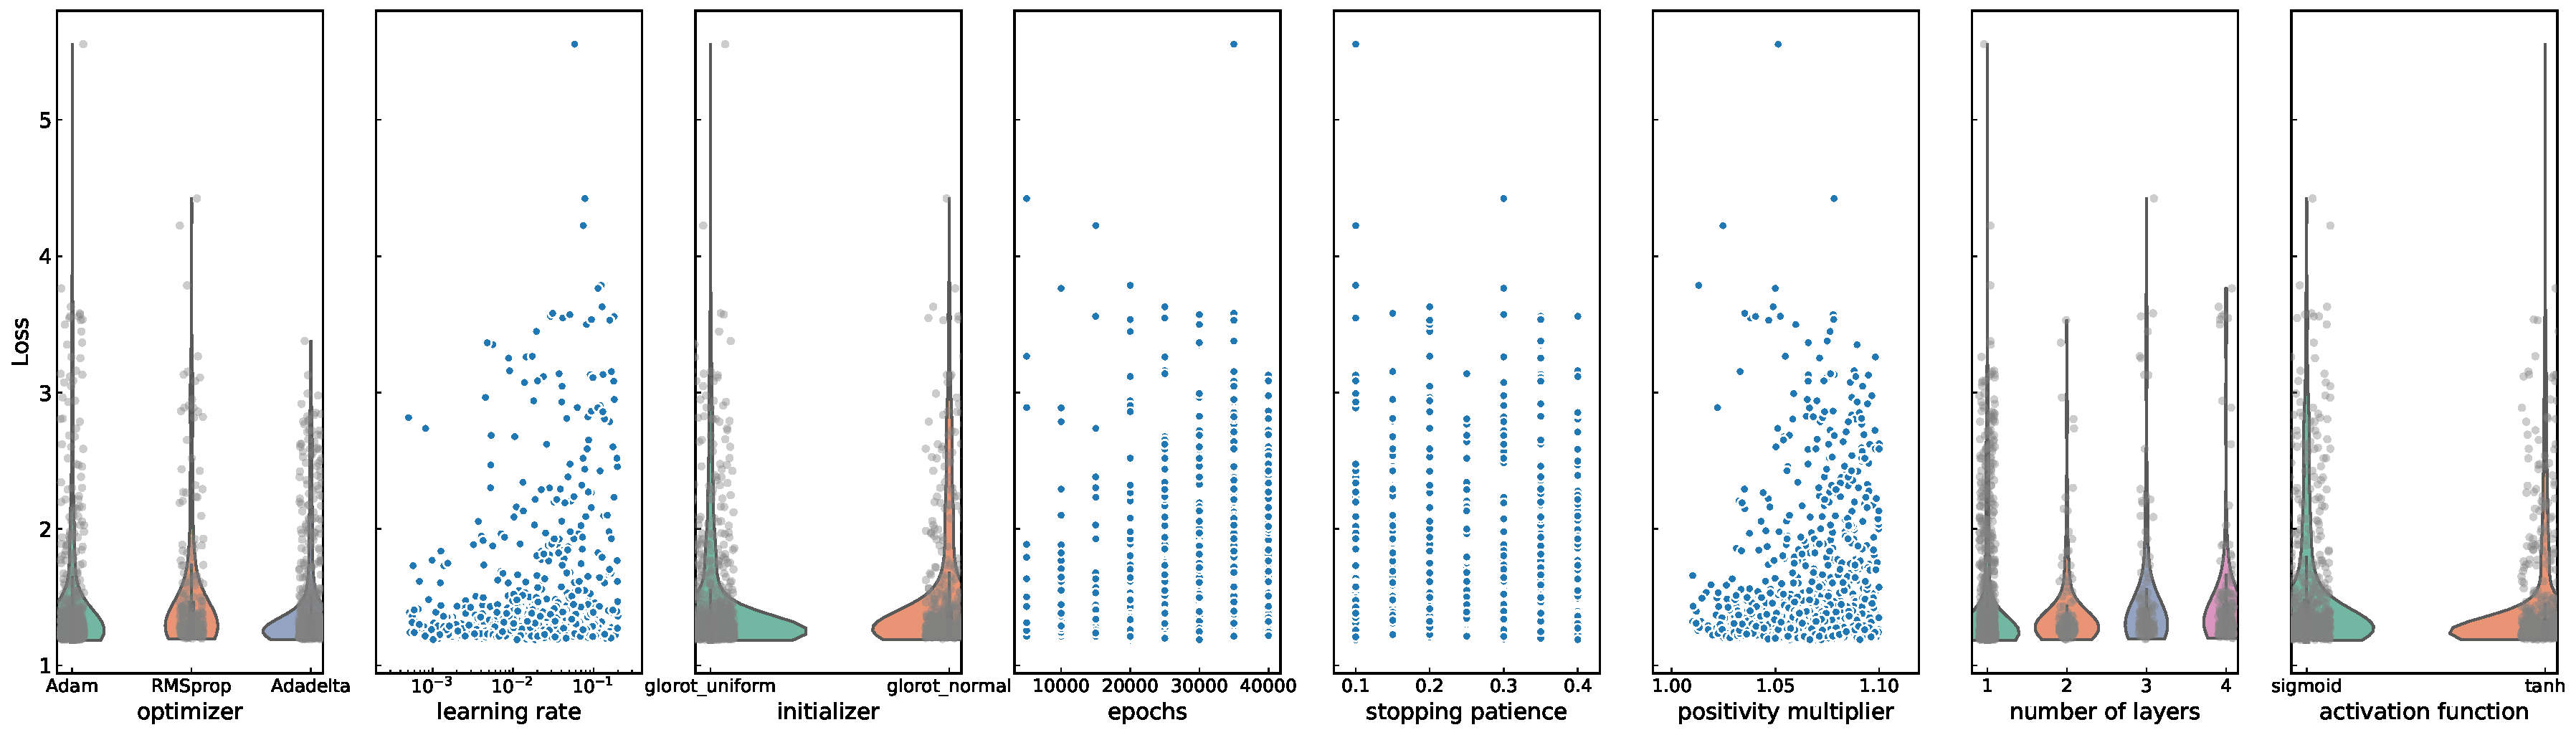
\includegraphics[width=\textwidth]{juan_future_hyperopt/dis-fullpage.pdf}
        Thousands of fits for the hyperoptimization algorithm to choose:

        \begin{columns} \small
            \column{0.35\paperwidth}
            \begin{itemize}
                \item[\bct] Optimizer
                \item[\bct] Initializer
                \item[\bct] Stopping Patience
                \item[\bct] Number of Layers
            \end{itemize}
            \column{0.35\paperwidth}
            \begin{itemize}
                \item[\bct] Learning Rate
                \item[\bct] Epochs
                \item[\bct] Positivity Multiplier
                \item[\bct] Activation Function
            \end{itemize}
        \end{columns}
    } \vfill
\end{frame}

\begin{frame}
    \frametitle{Hyperoptimization: reward and generalization}
    If we use as hyperoptimization targe the $\chi^{2}$ of the fitted data, we risk finding the hyperparameter set that
    better overfits.


    \vfill

    \begin{columns}
        \column{0.75\linewidth}
        We avoid this problem by adopting \textbf{$\boldsymbol{k}$-folding}:

        \begin{itemize}
            \item Divide the data into $k$ sets.
            \item Leave one set out and fit the $k-1$ sets left.
            \item Optimize the average $\chi^{2}$ of the $k$ non-fitted sets.
        \end{itemize}
        \column{0.25\linewidth}
        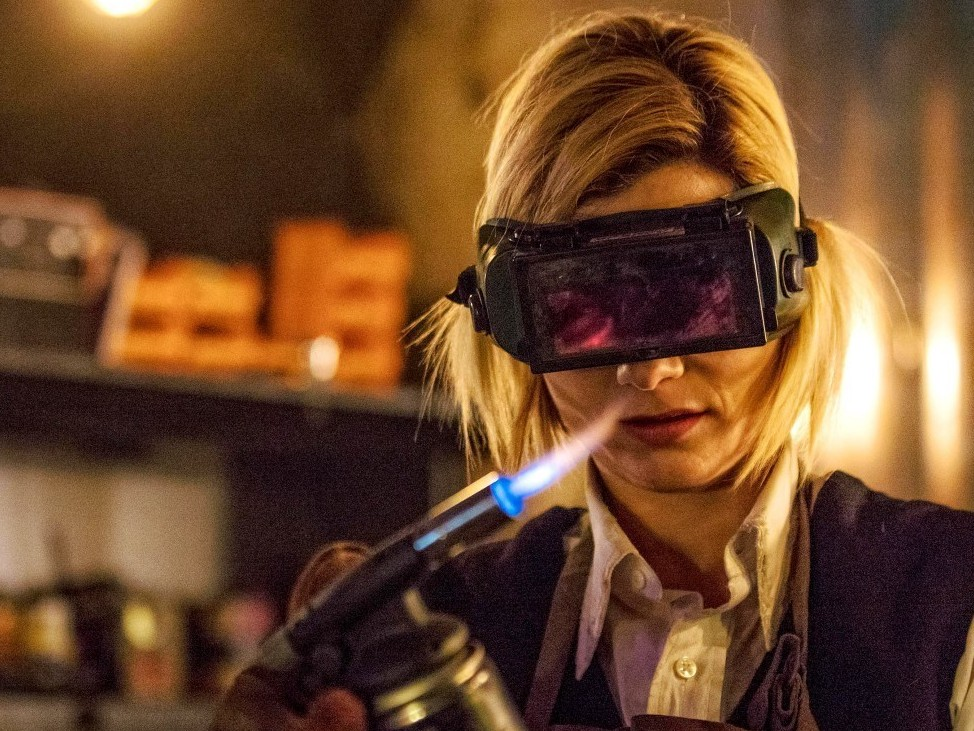
\includegraphics[width=\textwidth]{juan_future_hyperopt/doctor.jpg}
    \end{columns}

    \vspace{0.4cm}

    Example of function to hyperoptimize:

    \begin{equation*}
        \text{Loss}(optimizer\_name,\ depth\_of\_network) = \frac{1}{k}\displaystyle\sum^{i}_{k} \frac{\chi^{2}_{i}}{N_{i}}
    \end{equation*}

    Where we are computing the $\chi^{2}$ for the data that did not enter the fit. This ensures that the methodology
    can accomodate well even data that has never been seen by the fit.

\end{frame}
